\section{Metodología}
Con el fin de resolver las necesiades del ajedrez cuántico, se requiere el uso de una
red neuronal que pueda ser capaz de conocer, interpretar y usar los 
conceptos del ajedrez cuántico.

Para entender mejor la solución se ha 
planteado el siguiente gráfico que esquematiza 
el funcionamiento del sistema.

\begin{figure}
	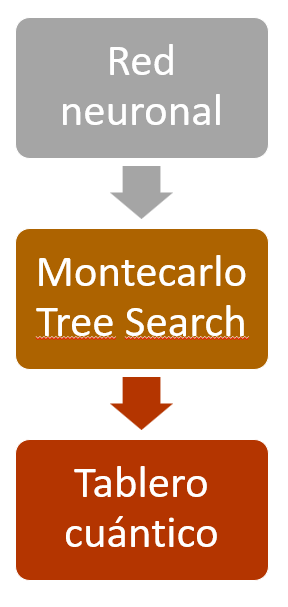
\includegraphics[width=5cm]{Imagenes/jerarquia_del_algoritmo.png}
\end{figure}

A continuación una breve descripción de cada componente del problema.

\subsection{Tablero Cuantico}
Sobre él se juegan las partidas, tiene implementadas las reglas de juego
necesarias para llevar a cabo el correcto desemvolvimiento del algoritmo inteligente,
ademas tiene en el las piezas que se usaran para las diversas situaciones de juego.
\subsection{Montecarlo Tree Search}
Encargado de hacer búsquedas en las jugadas para 
buscar las que tienen mejoresposibilidades de victoria, 
analisa dato pasados para poder cumplir con esta tarea
\subsection{Red Neuronal}
Encargado de tomar las desiciones en base de los 
analisis realizados a nivel del Montecarlo. Es el 
responsable de ordenar que es lo que se hace mientras 
avanza la partida de ajedrez que busca ganar el algoritmo.

